\documentclass{book}


% ==================================================================================================================================
% HEADER
% Documents packages, environements, page configuration

\usepackage[french]{babel}
\usepackage[T1]{fontenc}
\usepackage{ragged2e}
\usepackage{amsfonts}
\usepackage{systeme}
\usepackage{amsmath}
\usepackage{amssymb}
\usepackage{comment}
\usepackage{multicol}
\usepackage{lipsum} 
\usepackage{graphicx}
\usepackage{stmaryrd}
\usepackage{wrapfig}
\usepackage{colortbl}
\usepackage{cellspace}
\usepackage{ntheorem}
\usepackage{lmodern}
\usepackage{mathtools}
\usepackage{ragged2e}
\usepackage{tabularx}
\usepackage{titlepic}
\usepackage{fancyhdr}
\usepackage{caption}
\usepackage{xcolor}
\usepackage[linkbordercolor=white]{hyperref}
\usepackage[T1]{fontenc}
\usepackage{lmodern}
\usepackage{listings}
\usepackage{tikz}
\usepackage{tkz-graph}
\usepackage{pgfplots}
\usepackage{mdframed}
\usepackage{xparse}
\usepackage{enumitem}
\usepackage{titlesec}
\usepackage[top=3cm, bottom=3cm, left=3.5cm, right=3.5cm]{geometry}
\usepackage{etoolbox} % pour tester la présence d'un argument optionnel
\usepackage{subcaption}

% \pagestyle{empty}

\usetikzlibrary{cd}
\usetikzlibrary{patterns}
\usetikzlibrary{angles,quotes}
\usetikzlibrary{intersections, 3d, calc}

\usepgfplotslibrary{fillbetween}

\pgfplotsset{compat=1.18}


% - - - - - - - - - - - - - - - - - - - - - - - - - 
%                   PAGE SETTINGS
% - - - - - - - - - - - - - - - - - - - - - - - - - 

\setlength{\columnseprule}{1pt}               % ligne de séparation entre les colonnes
\def\columnseprulecolor{\color{black}}

\newcolumntype{C}{>{$\displaystyle}Sc<$}      % style d'affichage et taille 
\cellspacetoplimit=5pt                        % de la séparation entre colonnes
\cellspacebottomlimit=5pt

\renewcommand{\thechapter}{\arabic{chapter}}  % Set chapters numbers to 0

% Redéfinition de \part avec image optionnelle
\renewcommand{\part}[2][]{%
  \clearpage
  \refstepcounter{part} % incrémente le compteur de partie
  \addcontentsline{toc}{part}{\thepart\space #2} % ajoute au sommaire

  \begin{center}
    {\Huge\bfseries #2\par}
    \vspace{4em}  % Augmente l'écart à 2em
    \ifstrempty{#1}{}{%
      \includegraphics[width=0.4\textwidth]{#1}\par
    }
  \end{center}
  \vspace{2em}
}



% - - - - - - - - - - - - - - - - - - - - - - - - - 
%                 MATHS SHORTHANDS
% - - - - - - - - - - - - - - - - - - - - - - - - - 

\newcommand{\C}{\mathbb{C}}
\newcommand{\R}{\mathbb{R}}
\newcommand{\Q}{\mathbb{Q}}
\newcommand{\Z}{\mathbb{Z}}
\newcommand{\N}{\mathbb{N}}
\newcommand{\U}{\mathbb{U}}
\newcommand{\K}{\mathbb{K}}
\newcommand{\E}{\mathbb{E}}
\newcommand{\V}{\mathbb{V}}
\newcommand{\Lc}{\mathbb{L}}
\newcommand{\Fc}{\mathbb{F}}

\newcommand{\M}{\mathcal{M}}
\newcommand{\B}{\mathcal{B}}
\newcommand{\F}{\mathcal{F}}

%\renewcommand{\epsilon}{\varepsilon}
%\renewcommand{\phi}{\varphi}
%\renewcommand{\rho}{\varrho}

\renewcommand{\labelitemi}{\textbullet} % Utiliser des points noirs (•)

\newcommand{\myP}{\mathbb{P}}


% - - - - - - - - - - - - - - - - - - - - - - - - - 
%                 MODS NOTATION
% - - - - - - - - - - - - - - - - - - - - - - - - - 

\theorembodyfont{\upshape}

% Définir un environnement pour encadrer les définitions avec un titre
\NewDocumentEnvironment{definition}{O{}}
{
  \begin{mdframed}[linewidth=0pt,linecolor=gray,backgroundcolor=gray!10,roundcorner=5pt]
  \textbf{Définition}%
  \IfNoValueTF{#1}{}{~(\textbf{#1})} % Affiche le titre entre parenthèses et en gras s'il est fourni
  . % Point à la fin
}
{
  \end{mdframed}
}

% Définir un environnement pour encadrer les théorèmes avec un titre
\NewDocumentEnvironment{theorem}{O{}}
{
  \samepage
  \begin{mdframed}[linewidth=1pt,linecolor=darkgray,backgroundcolor=darkgray!10,roundcorner=5pt]
  \textbf{Théorème}%
  \IfNoValueTF{#1}{}{~(\textbf{#1})} % Affiche le titre entre parenthèses et en gras s'il est fourni
  . % Point à la fin
}
{
  \end{mdframed}
}

% Définir un environnement pour encadrer les corollaires
\NewDocumentEnvironment{corollary}{O{}}
{
  \begin{mdframed}[linewidth=1pt,linecolor=gray,backgroundcolor=gray!10,roundcorner=5pt]
  \textbf{Corollaire}%
  \IfNoValueTF{#1}{}{~(\textbf{#1})} % Affiche le titre entre parenthèses et en gras s'il est fourni
  . % Point à la fin
}
{
  \end{mdframed}
}


% Définir un environnement pour encadrer les critères
\NewDocumentEnvironment{criteria}{O{}}
  {
    \begin{mdframed}[linewidth=1pt,
                      linecolor=gray,
                      backgroundcolor=gray!10,
                      roundcorner=5pt
                      ]
    \textbf{Critère}%
    \IfNoValueTF{#1}{}{~(\textbf{#1})} % Affiche le titre entre parenthèses et en gras s'il est fourni
    . % Point à la fin
  }
  {
    \end{mdframed}
  }

% Définir un environnement pour encadrer les prorpiétés avec un titre
\NewDocumentEnvironment{prop}{O{}}
{
  \begin{mdframed}[linewidth=0pt,linecolor=gray,backgroundcolor=gray!10,roundcorner=5pt]
  \textbf{Propriété}%
  \IfNoValueTF{#1}{}{~(\textbf{#1})} % Affiche le titre entre parenthèses et en gras s'il est fourni
  . % Point à la fin
}
{
  \end{mdframed}
}
				

\theoremstyle{plain}
\newtheorem*{remark}{Remarque}
\newtheorem*{proposition}{Proposition}
\newtheorem*{lemma}{Lemme}
%\newtheorem*{prop}{Propriété}
\newtheorem*{proof}{Démonstration}
\newtheorem*{example}{Exemple}

% Créer un environnement qui empêche les coupures de page
\newenvironment{nobreakproposition}
{
  \par\begingroup\samepage % Empêcher les coupures de page
  \begin{proposition}
}
{
  \end{proposition}
  \par\endgroup
}


% - - - - - - - - - - - - - - - - - - - - - - - - - 
%             Itemize env settings
% - - - - - - - - - - - - - - - - - - - - - - - - - 

% \setlist[itemize,1]{label=\textbullet}
% \setlist[itemize,2]{label=\textbullet}
% \setlist[itemize,3]{label=\textbullet}
% \setlist[itemize,4]{label=\textbullet}


% - - - - - - - - - - - - - - - - - - - - - - - - - 
%             Tableofcontents settings
% - - - - - - - - - - - - - - - - - - - - - - - - - 


% % Profondeur des mini-tables des matières
% \setcounter{minitocdepth}{2}  % Jusqu’aux sous-sections
% \setcounter{parttocdepth}{1}  % Jusqu’aux chapitres dans les parties

% % Configurer l’apparence
% \mtcsetrules{minitoc}{off}  % Désactiver les lignes pour les chapitres
% \mtcsetrules{parttoc}{off}   % Désactiver les lignes pour les parties

% % Si tu veux que la table principale n'affiche que les parties :
% \setcounter{tocdepth}{-1}  % N'afficher que les \part dans la table principale


% - - - - - - - - - - - - - - - - - - - - - - - - - 
%                       TITLE
% - - - - - - - - - - - - - - - - - - - - - - - - - 


% ==================================================================================================================================
% Setting Title 

% Titre du document
\title{Révisions Master IMA}
\author{Axel PIGEON}
\date{\today}

\setlength{\parindent}{0pt}
\renewcommand{\labelitemi}{\textbullet} % Utiliser des points noirs (•)

\begin{document}


% ==================================================================================================================================
% CONTENT


% Page de titre 
\maketitle

% Table des matières 
\tableofcontents
\newpage

\setlength{\parindent}{0pt}

% Inclusion des chapitres 
\part{Probabilités}
\chapter{Espaces Probabilisés et Variables Aléatoires}

\justify

\setlength{\parindent}{0pt}
\renewcommand{\labelitemi}{\textbullet} % Utiliser des points noirs (•)

% ==================================================================================================================================
% Introduction 

% TODO : 
%     - Revoir définition variable aléatoire : https://mathieu-mansuy.fr/pdf/MP2I-Chapitre29.pdf 
%     - Déplacer lois d'une variable dans ce chapitre 
%     - Ajouter définition support 
%     - Rajouter propriétés vues dans le cours en ligne 
%     - Définition variables iid 
%     - Rajouter une partie indépendance 


% ==================================================================================================================================
% Espaces Probabilisés et Mesures 

\section{Espaces Probabilisés, Mesures et Variables Aléatoires}

\subsection{Univers}

Introduisons les concepts fondamentaux des probabilités, les univers et les espaces probabilisés. 

\begin{definition}[Univers]
    On appelle univers $\Omega$ pour une expérience aléatoire, l'ensemble de toutes les issues (situations finales) possibles 
    de cette expérience aléatoire. Chaque élément $ \omega \in \Omega$ représente une \textbf{issue} de cette expérience aléatoire.  
\end{definition}

\begin{example}
    \begin{itemize}
        \item Pour une expérience aléatoire de lancer de dé, il existe 6 issues possibles correspondant aux 6 faces du dé. 
        On a donc $\Omega = \{1, 2, 3, 4, 5, 6\}$. 
        \item Si on pioche un boule dans une urne contenant une boule rouge et deux boules noires, on a 
        $ \Omega = \{\text{rouge}, \text{noir}\}$. 
    \end{itemize}
\end{example}

A partir d'un univers, on peut définir la notion d'espace probabilisé. Plus complexe, la définition nécessaire les prérequis 
du cours d'intégration et de théorie de la mesure. 

\begin{definition}[Espace Probabilisé]
    Un espace probabilisé est un \textbf{triplet} $ (\Omega, \mathcal{F}, \myP)$ où :
    \begin{itemize}
        \item $\Omega$ est un univers. 
        \item $ \mathcal{F}$ est une tribu ($\sigma$-algèbre) sur $ \Omega$. 
        \item $ \myP$ est une mesure de probabilité sur $ \mathcal{F}$ (voir plus loin). 
    \end{itemize}
\end{definition}



\subsection{Évènements, Issues et Mesure de Probabilité }

\begin{definition}[Évènement]
    Soit $\Omega$ un univers. On définit un évènement de $\Omega$ comme un sous-ensemble $A \subseteq \Omega$. 
\end{definition}

\begin{remark}
    Comme définit au début, les \textbf{issues} $ \omega \in \Omega$ correspondent à des résultats élémentaires de l'expérience 
    aléatoire, à ne pas confondre avec les évènements. 
    Dans notre expérience de lancer de dé, $\{2\} \in \Omega$ est \textbf{l'issue} correspondant à "obtenir un 2" et 
    $A = \{1,2\} \subset \Omega$ est \textbf{l'évènement} correspondant à "le résultat est inférieur ou égal à 2". 
\end{remark}

Par construction, $ \mathcal{F}$ contient donc tous les évènements et issues possibles de l'expérience aléatoire. 
Elle est dont "plus complète" que $\Omega$, on retrouve les propriétés des espaces mesurables, vus en intégration en Licence. 

\begin{definition}[Mesure de Probabilité]
    Soit un espace probabilisé $(\Omega, \mathcal{F}, \myP)$. Une mesure de probabilité $ \myP$ 
    sur $ \mathcal{F}$ est une mesure (au sens de la théorie de la mesure) qui vérifie : 
    \begin{enumerate}
        \item $ \myP : \mathcal{F} \longrightarrow [0,1]$
        \item $ \myP(\Omega) = 1$ 
    \end{enumerate}
\end{definition}

\begin{remark}[Rappel : Mesure]
    Une fonction $ \mu : (X, \mathcal{B}) \longrightarrow \overline{\R_+}$ telle que : 
    \begin{enumerate}
        \item $ \mu(\emptyset) = 0 $ 
        \item \textbf{(Sigma-additivité)} : $ \forall (A_n)_{n \in \N}$ suite de parties mesures \textbf{deux à deux disjointes}, on ait : 
            \[ \mu \left( \bigcup_{n \in \N} A_n \right) = \sum_{n \in \N} \mu(A_n) \]
        est appelée mesure sur l'espace $(X, \mathcal{B}, \mu)$ alors appelé \textbf{espace mesuré}. 
    \end{enumerate}
\end{remark}

\section{Variable Aléatoire}

\subsection{Définition et Loi}

Pour pouvoir quantifier des calculs de probabilités ou ce que nous appellerons plus tard des lois, nous devons définir 
les variables aléatoires. 

\begin{definition}[Variable Aléatoire]
    Une variable aléatoire est une fonction mesurable qui associe une valeur numérique à chaque issue d'un espace probabilisé. 

    \vspace{0.5cm}

    Plus formellement, une variable aléatoire $X$ sur un espace probabilisé $(\Omega, \mathcal{F}, \myP)$ 
    est une fonction $ X : \Omega \longrightarrow \R$ telle que, pour tout ensemble $B \in \mathcal{B}_\R$ (tribu borélienne), 
    on ait $X^{-1} (B) \subset \mathcal{F}$. 

    \vspace{0.5cm}

    On définit l'ensemble des valeurs possibles de la variable aléatoire comme l'image de $\Omega$ par $X$ noté $X(\Omega)$. 
\end{definition}

La mesurabilité d'une variable aléatoire permet donc garantir que les évènements associés aux valeurs de la variable 
aléatoire sont bien mesurables par la mesure de probabilité. 

\vspace{0.5cm}

Maintenant que nous avons définit formellement le concept de variable aléatoire, on peut lier cette définition 
à celle des évènements. En effet, une variable aléatoire est une fonction mesurable sur un espace probabilisé $(\Omega, \mathcal{F}, \myP)$
telle que : 
    \[ X : \Omega \longrightarrow \R \quad \forall B \in \mathcal{B}_\R, X^{-1} (B) \subset \mathcal{F} \] 
On peut alors caractériser un évènement $A$ comme la préimage d'un sous-ensemble de $\R$ par $X$ de la façon suivante. 
    \[ A = X^{-1}(B) \; \text{pour un certain} \; B \in \mathcal{B}_\R \] 
D'où la définition suivante...

\begin{definition}[Evènement d'une expérience aléatoire]
    Soit $X$ une variable aléatoire réelle définie sur un univers $\Omega$. 
    On appelle évènement $[X = x]$ de l'expérience aléatoire l'ensemble des issues possibles correspondant à cet évènement $x \in \R$ . 
    Autrement dit :
        \[ [X = x] = \{w \in \Omega \; | \; X(\omega) = x\} = X^{-1}(x) \] 
\end{definition}

\begin{definition}[Loi]
    Soit $X$ une variable aléatoire. On appelle loi de $X$ la donnée de toutes les probabilités $ \myP(X = x)$ pour 
    tout $x \in X(\Omega)$.  
\end{definition}

Pour donner la loi d'une variable aléatoire, il faut d'abord déterminer le support de la variable aléatoire puis en suite 
calculer la probabilité de chaque issue. 
On note le résultat dans un tableau pour plus de praticité. 

\begin{example}
    Soit l'exprérience aléatoire du lancer d'un dé à 6 faces non truqué. On a :
        \[ \Omega = \{1,2,3,4,5,6\} \]
    Nous nous trouvons dans une situation d'équiprobabilité d'où :
        \[ \forall x \in X(\Omega), \quad \myP(X = x) = \frac{1}{6} \]
    D'où le tableau suivant :
    \begin{center}
        \begin{tabular}{c|c|c|c|c|c|c}
            $\Omega$ & 1 & 2 & 3 & 4 & 5 & 6 \\
            \hline 
            $ \myP(X = x)$ & $\frac{1}{6}$ & $\frac{1}{6}$ & $\frac{1}{6}$ & $\frac{1}{6}$ & $\frac{1}{6}$ & $\frac{1}{6}$ \\ 
        \end{tabular}
    \end{center}  
\end{example}

\subsection{Variables Discrètes et Continues}

Selon la nature de l'espérience aléatoire et de l'univers choisis, on distingue deux grands types de variables aléatoires : 
les variables aléatoires \textbf{discrètes} et \textbf{continues}. Cette distinction est fondamentale car elle 
caractérise la façon dont on exprime et calcule ensuite les probabilités.

\begin{definition}[Variable aléatoire discrète]
    Une variable aléatoire $X$ définie sur un espace probabilisé $(\Omega, \mathcal{F}, \myP)$ est dite 
    \textbf{discrète} si l'ensemble de ses valeurs possibles $X(\Omega)$ est un ensemble \textbf{fini ou dénombrable}. 
    Dans ce cas, la loi de probabilité de $X$ est donnée par une fonction de masse et les probabilités 
    s'expriment comme des sommes. 
\end{definition}

\begin{example}
    Le résultat d'un lancer de dé est une variable aléatoire discrète. 
    Par exemple, si $X$ désigne le résultat d’un lancer de dé, alors $X(\Omega) = \{1,2,3,4,5,6\}$.
\end{example}

\begin{definition}[Variable aléatoire continue]
    Une variable aléatoire $X$ est dite \textbf{continue} si elle peut prendre une infinité non dénombrable de valeurs, typiquement un intervalle de $\R$. 
    Dans ce cas, il n'existe pas de fonction de masse mais une \textbf{densité de probabilité}, et les probabilités s'expriment 
    par des \textbf{intégrales}.
\end{definition}


\begin{example}
    Le temps d'attente avant un événement (modélisé par une loi exponentielle), ou la taille d'une personne (loi normale), 
    sont des variables continues. Si $X$ est la taille d’un individu, alors $X(\Omega) \subseteq \R$ est un intervalle de réels.
\end{example}

\begin{remark}
    La distinction entre lois discrètes et lois continues repose donc sur la nature de la mesure de probabilité utilisée :
    \begin{itemize}
        \item \textbf{Mesure de comptage} (ou somme de Dirac) $\Rightarrow$ lois discrètes.
        \item \textbf{Mesure de Lebesgue} (avec densité) $\Rightarrow$ lois continues.
    \end{itemize}
\end{remark}

Nous allons maintenant étudier les deux grands types de lois de probabilité selon la nature de la variable aléatoire : 

\begin{itemize}
    \item Dans le cas discret : lois binomiale, géométrique, de Poisson...
    \item Dans le cas continu : loi uniforme, loi exponentielle, loi normale...
\end{itemize}

\chapter{Variables Aléatoires Réelles Discrètes}

\justify

\setlength{\parindent}{0pt}
\renewcommand{\labelitemi}{\textbullet} % Utiliser des points noirs (•)

% ==================================================================================================================================
% Introduction 


% ==================================================================================================================================
% Variables Aléatoires Réelles Discrètes


\section{Espérance, Variance et Écart-type}

\begin{definition}[Espérance]
    Soit $X : \Omega \longrightarrow \R$ une variable aléatoire discrète. 
    On appelle espérance l'application $ \E : X(\Omega) \longrightarrow \R $ qui calcule la moyenne de $X$ pondérée par les valeurs qu'elle prend. 
    Plus formellement :
        \[ \boxed { \E(X) = \sum_{x \in X(\Omega)} x \myP(X = x) }\] 
\end{definition}

\begin{prop}[Espérance]
    L'espérance est une fonction linéaire. Autrement dit, pour toutes variables aléatoires $X,Y$ sur  un univers $\Omega$, 
    et pour tout $a,b \in \R$, on a :
        \[ \E(X+Y) = \E(X) + \E(Y) \quad \E(aX + b) = a\E(X) + b \]
\end{prop}

Lors d'une expérience aléatoire, par exemple un jeu d'argent l'espérance représente le gain moyen d'un joueur par partie 
s'il joue un grand nombre de fois. Son signe permet de savoir si le jeu est dit équitable (autant de chances de gagner que 
de perdre). 

\vspace{0.3cm}

Il peut souvent arriver que l'on veuille appliquer une fonction à notre variable aléatoire. 
Un théorème nous permet alors simplement de calculer l'espérance de cette "nouvelle" variable aléatoire. 

\begin{theorem}[Transfert]
    Soit $X$ une variable aléatoire discrète sur un univers $\Omega$ et $g : \R \longrightarrow \R$ une application. 
    L'espérance de la variable aléatoire $g(X) : \Omega \longrightarrow \R$ est l'application $ \E(g(X)) : \mathcal{F}(\Omega) \longrightarrow \R$ 
    telle que : 
        \[ \boxed{ \E(g(X)) = \sum_{x \in X(\Omega)} g(x) \myP(X = x) } \]  
\end{theorem}

\begin{definition}[Variance et écart-type]
    Soit $X$ une variable aléatoire discrète sur un univers $\Omega$. On appelle variance l'application 
    $\V : X(\Omega) \longrightarrow \R$ telle que :
        \[ \boxed { \V(X) = \sum_{x \in X(\Omega)} (x - \E(X))^2 \myP(X = x) } \]
    De même, on appelle écart type l'application $ \sigma : X(\Omega) \longrightarrow \R$ telle que : 
        \[ \boxed{ \sigma(X) = \sqrt{\V(X)} } \]  
\end{definition}

La variance permet de mesurer la dispersion de la variable aléatoire autour de son espérance. 

\begin{remark}
    Les notions d'espérance, variance et écart-type sont définies par des sommes potentiellement infinies. 
    Il se peut donc que dans le cas de variables aléatoires définies sur des univers infinis, leur espérance, 
    variance et écart-type n'existent pas. Une étude de convergence de la somme est donc judicieuse. 
    En revanche pour les variables aléatoires définies sur un univers fini ces valeurs existent bien. 
\end{remark}

\begin{theorem}[Formule de König-Huygens]
    Soit $X$ une variable aléatoire sur un univers $\Omega$ fini. On a alors : 
        \[ \boxed{ \V(X) = \E(X^2) - \E(X)^2 } \]
\end{theorem}

\begin{remark}
    Le calcul de la variance d'une variable aléatoire réelle finie est donc assez facile quand on le met en relation 
    avec la formule de König-Huygens et la formule du transfert...
\end{remark}

A partir de toutes ces formules, on peut en déduire quelques propriétés sympatiques sur la variance :

\begin{prop}[Variance]
    Soit $X$ une variable aléatoire finie et $a,b \in \R$, on a :
        \[ \V(aX+b) = a^2 \V(X) \quad \V(X + b) = \V(X) \]
    La variance est donc assez similaire à une forme quadratique et est invariante par translation. 
    De plus, la variance d'une variable aléatoire est invariable par translation des valeurs de la variable aléatoire. 
\end{prop}

\begin{theorem}[Inégalité de Markov]
    Si $X$ est une variable aléatoire réelle discrète \textbf{positive} ou nulle sur $\Omega$ d'espérance $\E(X)$, alors :
        \[ \forall a \in ]0, + \infty [ \quad P(X \geqslant a) \leqslant \dfrac{\E(X)}{a} \]
    Cela fournit un majorant de la probabilité que $X$ dépasse un seuil $a$ donné.
    Ce résultat est particulièrement utile pour borner des queues de distributions sans connaître leur loi exacte.
\end{theorem}


\section{Principales Lois}

Abordons en détail maintenant quelques lois usuelles à connaître sur le bout des doigts. 
Ces lois permettent de modéliser la plupart des expériences aléatoires. 

\subsection{Loi Uniforme}

\begin{definition}[Loi Uniforme]
    Soit $n \in \N^*$. On dit qu'un variable aléatoire $X$ suit une \textbf{loi uniforme} sur $ \llbracket 1, n \rrbracket $ 
    lorsque son support est $X(\Omega) = \llbracket 1, n \rrbracket $ et chaque issue a la même probabilité de se produire. 
    Autrement dit : 
        \[ \forall x \in \llbracket 1, n \rrbracket, \quad P(X = x) = \frac{1}{n} \]
    On note alors $X \sim \mathcal{U}(\llbracket 1, n \rrbracket)$. 
\end{definition}

\begin{proposition}
    Soit $X \sim \mathcal{U}(\llbracket 1, n \rrbracket)$ alors l'espérance et la variance de $X$ sont de la forme : 
        \[ \E(X) = \frac{n+1}{2} \quad \text{et} \quad \V(X) = \frac{n^2-1}{12}  \] 
\end{proposition}

\subsection{Loi de Bernoulli}

\begin{definition}[Loi de Bernoulli]
    Une variable aléatoire $X$ suit une \textbf{loi de Bernoulli} de paramètre $p \in ]0,1[$ si il n'existe que deux issues 
    possibles $X(\Omega) = \{ 0,1 \}$ telles que : 
        \[ \myP(X = 1) = p \quad \text{et} \quad \myP(X = 0) = 1 - p \] 
    On note alors $X \sim \mathcal{B}(p)$.  
\end{definition}

\begin{proposition}
    Soit $X \sim \mathcal{B}(p)$ alors l'espérance et la variance de $X$ sont de la forme :
        \[ \E(X) = p \quad \text{et} \quad \V(X) = p(1-p)  \] 
\end{proposition}

\subsection{Loi Binomiale}

L'expérience aléatoire consistant à répéter $n \in \N$ fois une expérience de Bernoulli de paramètre $ p \in ]0,1[$
de {manière indépendante} est appelée \textbf{schéma de Bernoulli} de paramètres $n$ et $p$. 

\begin{definition}[Loi Binomiale]
    La variable aléatoire $X$ égale au \textbf{nombre de succès} d'un schéma de Bernoulli suit une {loi binomiale} 
    de paramètres $n$ et $p$. 

    On note alors $X \sim \mathcal{B}(n,p)$. 
\end{definition}

\begin{proposition}
    Soit $X \sim \mathcal{B}(n,p)$. On a alors $X(\Omega) = \llbracket 0, n \rrbracket$ et pour tout $k \in \N$ tel que 
    $0 \leqslant k \leqslant n $, {la probabilité d'obtenir $k$ succès} est donnée par :
        \[ \myP(X = k) = \binom{n}{k} \times p^k \times (1-p)^{n-k}  \] 
\end{proposition}

\begin{proposition}
    Soit $X \sim \mathcal{B}(n,p)$ alors l'espérance et la variance de $X$ sont de la forme :
        \[ \E(X) = np \quad \text{et} \quad \V(X) = np(1-p)  \] 
\end{proposition}

\subsection{Loi géométrique}

\begin{definition}[Loi géométrique]
    Une variable aléatoire $X$ suit une loi géométrique de paramètre $p \in ]0,1[$ lorsque $X(\Omega) = \N^*$ et que 
        \[ \forall k \in \N^*, \quad \myP(X = k) = p(1-p)^{k-1}  \] 
    On note alors $X \sim \mathcal{G}(p)$. 
\end{definition}

Une loi géométrique représente le temps d'attendre du premier succès d'un espérience de Bernoulli. 
Autrement dit X est le rang de l'épreuve ayant mené au premier succès. 

\begin{proposition}
    Soit $X \sim \mathcal{G}(p)$ où $p \in ]0,1[$ l'espérance et la variance de $X$ sont de la forme :
        \[ \E(X) = \frac{1}{p} \quad \text{et} \quad \V(X) = \frac{1-p}{p^2} \] 
\end{proposition}

\subsection{Loi de Poisson}

\begin{definition}[Loi de Poisson]
    Une variable aléatoire $X$ suit une loi de Poisson de paramètre $\lambda > 0$ lorsque $X(\Omega) = \N$ et 
        \[ \forall k \in \N, \quad P(X = k) = e^{- \lambda} \times \frac{\lambda^k}{k!} \]  
    On note alors $ X \sim \mathcal{P}(\lambda)$. 
\end{definition}

Une loi de Poisson modélise le nombre d'événements se produisant dans un intervalle de temps ou d’espace donné, lorsque ces événements sont rares et indépendants.
Par exemple, elle peut modéliser le nombre de voitures passant par un péage en une journée, ou le nombre de fautes de frappe sur une page de texte.

\begin{proposition}
    Soit $ X \sim \mathcal{P}(\lambda)$ alors l'espérance et la variance de $X$ sont de la forme :
        \[ \E(X) = \lambda \quad \text{et} \quad \V(X) = \lambda  \] 
\end{proposition}

\subsection*{Résumé des lois discrètes usuelles}

\begin{center}
    \begin{tabular}{|c|c|c|c|}
        \hline
        \textbf{Loi} & \textbf{Support} & \textbf{Espérance $\E(X)$} & \textbf{Variance $\V(X)$} \\
        \hline
        $\mathcal{U}(\llbracket 1, n \rrbracket)$ & $\llbracket 1, n \rrbracket$ & $\frac{n+1}{2}$ & $\frac{n^2 - 1}{12}$ \\
        \hline
        $\mathcal{B}(p)$ & $\{0,1\}$ & $p$ & $p(1-p)$ \\
        \hline
        $\mathcal{B}(n, p)$ & $\llbracket 0, n \rrbracket$ & $np$ & $np(1-p)$ \\
        \hline
        $\mathcal{G}(p)$ & $\N^*$ & $\frac{1}{p}$ & $\frac{1-p}{p^2}$ \\
        \hline
        $\mathcal{P}(\lambda)$ & $\N$ & $\lambda$ & $\lambda$ \\
        \hline
    \end{tabular}
\end{center}


Les lois étudiées jusque-là sont toutes des lois discrètes, c’est-à-dire que la variable aléatoire prend un nombre fini ou dénombrable de valeurs.  
Dans de nombreux cas, on souhaite modéliser des phénomènes à valeurs continues (comme une durée, une taille, une température, etc.).  
Nous allons maintenant introduire les lois continues les plus classiques : loi uniforme, loi exponentielle, loi normale, etc.


\chapter{Variables Aléatoires Réelles Continues}

\justify

\setlength{\parindent}{0pt}
\renewcommand{\labelitemi}{\textbullet} % Utiliser des points noirs (•)

% ==================================================================================================================================
% Introduction 

On s'intéresse maintenant à des variables aléatoires qui prennent des valeurs réelles mais pas forcément en nombre fini ou dénombrable.
Il est donc nécessaire de définir une probabilité sur $\R$ telle que la probabilité des singletons soit nulle.
Pour cela, nous allons très fortement nous appuyer sur l'intégrale de Lebesgue et la théorie de la mesure. 

% ==================================================================================================================================
% Généralités

\section{Généralités}

\subsection{Vers les variables aléatoires continues}

Dans les chapitres précédents, nous avons vu comment construire, à partir d'univers, des espaces probabilisés 
muni d'une tribu (structure mesurable) et d'une mesure de probabilité. Dans ce cadre probabiliste, une mesure particulière 
joue un rôle significatif sur $\R$ : la \textbf{mesure de Lebesgue}. 

Il est temps maintetant de définir les variables aléatoires réelles continues, c'est à dire, 
des fonctions mesurables dont la loi de probabilité est absolument continue par rapport à la mesure de Lebesgue. 
Intuitivement, cela signifie que nous seront capable de calculer des probabilités par une densité : une fonction intégrable 
positive sur $\R$ dont l'intégrale vaut 1 et permettant de calculer des probabilités par intégration. 

Ceci nécessitera l’introduction de quelques outils d’analyse (densité, intégration, espérance sous forme intégrale), 
qui généraliseront les formules que nous avions pour les lois discrètes.

\subsection{Définitions et propriétés}

\begin{definition}[Variable aléatoire continue]
    Une variable aléatoire $X$ est dite \textbf{continue} si elle peut prendre une infinité non dénombrable de valeurs, typiquement un intervalle de $\R$. 
    C'est donc une application $X : (\Omega, \mathcal{F}) \longrightarrow (\R, \mathcal{B}_\R)$ mesurable. 
        \[ \text{i.e} \quad \forall B \in \mathcal{B}_\R, \quad X^{-1}(B) \in \mathcal{F} \] 
\end{definition}

On peut donc appliquer la mesure de probabilité $\myP$ aux évènements de la forme $\{\omega \in \Omega\}$. 

\begin{definition}[Loi d'une variable aléatoire réelle continue]
    La loi d'une variable aléatoire continue $X$ est définie comme la \textbf{mesure image} de $ \myP$ par $X$ notée 
    $ \myP_X$ telle que : 
        \[ \forall B \in \mathcal{B}_\R, \quad \myP_X(B) = \myP(X^{-1}(B)) = \myP \left( \{\omega \in \Omega \; | \; X(\omega) \in B\} \right) \] 
    Cette loi permet donc de calculer la probabilité que la variable $X$ soit dans un intervalle $[a,b] \subseteq \R$ 
    de la façon suivante : 
        \[ \myP(a < X \leqslant b) = \myP(\{X \in ]a,b]\}) = \myP_X(]a,b]) \]  
\end{definition}

\begin{definition}[Densité de Probabilité]
    Si la mesure $\myP_X$ est absoluement continue par rapport à la mesure de Lebesgue sur $\R$ on dit 
    que $X$ admet une \textbf{densité de probabilité} $ f : \R \longrightarrow \R_+ $ telle que : 
        \[ \forall B \in \mathcal{B}_\R, \quad \myP_X(B) = \int_B f(x) \; dx \] 
\end{definition}


\subsection{Fonction de répartition}

\begin{definition}[Fonction de répartition]
    Soit $X$ une variable aléatoire réelle continue. Sa {fonction de répartition} $F_X$ est définie par :
    \[ F_X : 
        \begin{cases}
            \R \longrightarrow [0,1] \\ 
            a \longmapsto F_X(B) = \myP(X \leqslant a)
        \end{cases} \]
    $F_X$ est une fonction croissante admettant la limite $0$ en $- \infty$ et la 
    limite $1$ en $+ \infty$ et elle est continue à droite. 
\end{definition}

\begin{proposition}[Lien avec la densité]
    Si $X$ admet une densité de probabilité $f$, alors $F_X$ est dérivable et :
        \[
            F_X'(x) = f(x), \quad \text{pour presque tout } x \in \R.
        \]
    On a aussi, pour tout $a < b$ :
        \[
            \myP(a < X \leqslant b) = F_X(b) - F_X(a).
        \]
\end{proposition}

\subsection{Propriétés des variables aléatoires continues}

\begin{definition}[Espérance]
    Soit $X$ une variable aléatoire continue réelle continue de densité $f_X$.
    On appelle espérance de $X$ le nombre 
        \[ \E(X) = \int_{\R} t f_X(t) dt \]
    Si cette intégrale est finie, on dit que l'espérance de $X$ existe. Dans le cas contraire, 
    on dit que la variable aléatoire $X$ n'a pas d'espérance. 
    Autrement dit, on dit que $X$ admet une espérance si l'intégrale $\displaystyle \int_{\R} t f_X(t) \; dt$ 
    est absolument convergente. 
\end{definition}

\begin{theorem}[Formule de Transfert]
    Soit $X$ une variable aléatoire réelle continue de densité $f_X$, et $\varphi : \R \to \R$ une fonction mesurable telle que l’intégrale $\displaystyle \int_{\R} |\varphi(t)| f_X(t) dt$ soit finie. Alors :
        \[ \E(\varphi(X)) = \int_{\R} \varphi (t)f_X(t) dt\]
    Cette formule est une généralisation de l'espérance, on peut par exemple calculer $\E(\ln X)$, $\E(X^2)$, ...
\end{theorem}

\begin{definition}[Variance]
    Soit $X$ une variable aléatoire admettant une espérance. La variance de $X$ est le nombre :
        \[ V(X) = E((X - E(X))^2) = \int_{\R} (t - E(X))^2 f_X(t) \; dt \]
    Toujours comme chez les variables aléatoires réelles discrètes, l'écart-type de $X$ est la racine carrée de $V(X)$ si $V(X)$ existe.
\end{definition}

\begin{theorem}[Koenig-Huyghens]
    Ce théorème permet de calculer plus simplement la variance, à condition que l’espérance $E(X)$ et $E(X^2)$ existent :
        \[ V(X) = E(X^2) - E(X)^2 \]
    C’est souvent la méthode la plus directe pour déterminer la variance d’une variable aléatoire continue.
\end{theorem}


% ==================================================================================================================================
% Principales Lois

\section{Principales Lois}

Définissons maintenant quelques lois fondamentales à connaître par coeur...

\subsection{Loi Uniforme}

\begin{definition}[Loi Uniforme]
    Une variable aléatoire continue $X$ suit une loi uniforme sur $[a,b] \subseteq \R$ lorsque sa densité $f$ 
    est une fonction porte sur l'intervalle $[a,b]$. 
        \[ \text{i.e} \quad f : 
            \begin{cases}
                \R \longrightarrow [0,1] \\ 
                t \longmapsto   \begin{cases}
                                    \frac{1}{b-a} \; \text{si} \; t \in [a,b] \\ 
                                    0 \text{ sinon}
                                \end{cases}
            \end{cases} \] 
    On note alors $X \sim \mathcal{U}([a,b])$. 
\end{definition}

Ces variables aléatoires généralisent la notion d'équiprobabilité dans des espaces continus. 

\begin{proposition}
    Si $X \sim \mathcal{U}([a,b])$, alors la fonction de répartition de $X$ est donnée par : 
        \[ F_X(t) = 
            \begin{cases}
                0 \; \text{si} \; t < a \\ 
                \frac{t-a}{b-a} \; \text{si} \; t \in [a,b] \\ 
                1 \; \text{si} \; t > b 
            \end{cases} \] 
    De plus, on a : 
        \[ \E(X) = \frac{a + b}{2} \quad V(X) = \frac{(b-a)^2}{12} \] 
\end{proposition}


\subsection{Loi Exponentielle}

\begin{definition}[Loi Exponentielle]
    Soit $X$ une variable aléatoire continue. On dit que $X$ suit une loi exponentielle de paramètre $ \lambda > 0$ 
    si sa densité de probabilité est de la forme : 
        \[ f : 
            \begin{cases}
                \R \longrightarrow [0,1] \\ 
                t \longmapsto 
                    \begin{cases}
                        \lambda e^{-\lambda t} \; \text{si} \; t \geqslant 0 \\ 
                        0 \; \text{si} \; t \leqslant 0 
                    \end{cases}
            \end{cases} \] 
    On note alors $X \sim \mathcal{E}(\lambda)$. 
\end{definition}

Une loi exponentielle modélise la durée de vie d'une phénomène sans mémoire. Autrement dit, elle mesure la probabilité 
d'une phénomène ait duré pendant $t$ unités de temps. 

\begin{proposition}
    Si $X \sim \mathcal{E}(\lambda)$, alors sa fonction de répartition est donnée par : 
        \[ F_X(t) = 
            \begin{cases}
                1 - e ^{- \lambda t } \; \text{si} t \geqslant 0 \\ 
                0 \; \text{si} \; t < 0 
            \end{cases} \] 
    De plus, on a : 
        \[ \E(X) = \frac{1}{\lambda} \quad V(X) = \frac{1}{\lambda^2} \] 
\end{proposition}

\begin{figure}[h]
    \centering
    \begin{tikzpicture}
        \begin{axis}[
            domain=0:5,
            samples=100,
            axis lines=middle,
            xlabel=$t$,
            ylabel={$f_X(t)$},
            xtick={0,1,2,3,4,5},
            ytick=\empty,
            height=6cm,
            width=12cm,
            enlargelimits=false,
            clip=false,
            axis on top,
            grid=major,
        ]
            % Paramètre lambda
            \def\lambda{1}

            % Courbe de densité exponentielle
            \addplot [
                thick,
                blue,
                smooth
            ] {\lambda * exp(-\lambda * x)};

            % Zone entre 0 et espérance = 1/lambda
            \addplot [
                domain=0:1,
                samples=50,
                fill=blue!30,
                draw=none
            ] {\lambda * exp(-\lambda * x)} \closedcycle;

            % Lignes verticales
            \draw[dashed] (axis cs:1,0) -- (axis cs:1,{exp(-1)});
            \node[below] at (axis cs:1,0) {$\frac{1}{\lambda}$};
            \node[below] at (axis cs:0,0) {$0$};
        \end{axis}
    \end{tikzpicture}
    \caption{Densité de probabilité de la loi exponentielle $\mathcal{E}(\lambda)$ avec espérance $\frac{1}{\lambda}$}
\end{figure}



\subsection{Loi Normale}

\begin{definition}[Loi Normale]
    Soit $X$ une variable aléatoire continue. On dit que $X$ suit une loi normale de paramètres $\mu \in \R$ et $\sigma > 0$ 
    si sa densité de probabilité est donnée par : 
        \[ f : 
            \begin{cases}
                \R \longrightarrow \R^+ \\
                t \longmapsto \dfrac{1}{\sigma \sqrt{2\pi}} \exp\left( -\dfrac{(t - \mu)^2}{2\sigma^2} \right)
            \end{cases} \]
    On note alors $X \sim \mathcal{N}(\mu, \sigma^2)$. 
\end{definition}

La loi normale est très utilisée pour modéliser des phénomènes aléatoires centrés autour d'une moyenne $\mu$, 
avec une variabilité mesurée par l’écart-type $\sigma$. Elle est également appelée loi de Gauss.

\begin{proposition}
    Si $X \sim \mathcal{N}(\mu, \sigma^2)$, alors :
        \[ \E(X) = \mu \quad \text{et} \quad V(X) = \sigma^2 \]
    Sa fonction de répartition $F_X(t) = \mathbb{P}(X \leqslant t)$ n’a pas d’expression simple à l’aide de fonctions élémentaires. On utilise donc souvent la loi normale centrée réduite :
        \[ Z \sim \mathcal{N}(0, 1) \]
    avec densité : 
        \[ f_Z(t) = \dfrac{1}{\sqrt{2\pi}} e^{-t^2/2} \]
    et on a :
        \[ \mathbb{P}(X \leqslant t) = \mathbb{P}\left(Z \leq \dfrac{t - \mu}{\sigma}\right) \]
\end{proposition}

\begin{figure}[h]
    \centering
    \begin{tikzpicture}
        \begin{axis}[
            domain=-4:4,
            samples=100,
            axis lines=middle,
            xlabel=$x$,
            ylabel={$f_X(x)$},
            xtick={-3,-2,-1,0,1,2,3},
            ytick=\empty,
            height=6cm,
            width=12cm,
            enlargelimits=false,
            clip=false,
            axis on top,
            grid = major,
        ]
            % Densité normale centrée réduite
            \addplot [thick, blue, smooth] {1/sqrt(2*pi) * exp(-x^2/2)};
            
            % Zone entre -1 et 1 (mu - sigma, mu + sigma)
            \addplot [
                domain=-1:1, 
                samples=50,
                fill=blue!30,
                draw=none
            ] {1/sqrt(2*pi) * exp(-x^2/2)} \closedcycle;
            
            % Lignes verticales pour mu-sigma et mu+sigma
            \draw[dashed] (axis cs:-1,0) -- (axis cs:-1,0.25);
            \draw[dashed] (axis cs:1,0) -- (axis cs:1,0.25);
            
            % Flèche vers mu
            \node[below] at (axis cs:0,0) {$\mu$};
            \node[below] at (axis cs:-1,0) {$\mu - \sigma$};
            \node[below] at (axis cs:1,0) {$\mu + \sigma$};
        \end{axis}
    \end{tikzpicture}
    \caption{Densité de probabilité d'une loi normale $\mathcal{N}(\mu, \sigma^2)$ avec mise en évidence de l'intervalle $[\mu - \sigma, \mu + \sigma]$}
\end{figure}

\subsection{Loi de Cauchy}

\begin{definition}[Loi de Cauchy]
    Une variable aléatoire $X$ suit une loi de Cauchy de paramètre $x_0 \in \R$ (localisation) et $\gamma > 0$ (échelle) si :
        \[ f(t) = \frac{1}{\pi \gamma} \cdot \frac{1}{1 + \left( \frac{t - x_0}{\gamma} \right)^2} \]
    On note $X \sim \mathcal{C}(x_0, \gamma)$.
\end{definition}

La loi de Cauchy est une loi sans espérance ni variance, utilisée en physique (résonances).

\begin{proposition}
    La fonction de répartition de $X \sim \mathcal{C}(x_0, \gamma)$ est :
        \[ F_X(t) = \frac{1}{\pi} \arctan\left( \frac{t - x_0}{\gamma} \right) + \frac{1}{2} \]
\end{proposition}


\subsection{Loi Gamma}

\begin{definition}[Loi Gamma]
    Une variable aléatoire $X$ suit une loi Gamma de paramètres $k > 0$ (forme) et $\lambda > 0$ (taux) si :
        \[ f(t) = 
            \begin{cases}
                \dfrac{\lambda^k}{\Gamma(k)} t^{k-1} e^{-\lambda t} & \text{si } t \geq 0 \\
                0 & \text{sinon}
            \end{cases} \]
    On note $X \sim \Gamma(k, \lambda)$.
\end{definition}

La loi Gamma modélise des durées de vie cumulées (somme de $k$ exponentielles).

\begin{proposition}
    \[ \E(X) = \frac{k}{\lambda} \quad V(X) = \frac{k}{\lambda^2} \]
\end{proposition}


\subsection{Loi de Rayleigh}

\begin{definition}[Loi de Rayleigh]
    Une variable aléatoire $X$ suit une loi de Rayleigh de paramètre $\sigma > 0$ si sa densité est :
        \[ f(t) = 
            \begin{cases}
                \dfrac{t}{\sigma^2} e^{-t^2 / (2 \sigma^2)} & \text{si } t \geq 0 \\
                0 & \text{sinon}
            \end{cases} \]
    On note $X \sim \mathcal{R}(\sigma)$.
\end{definition}

\begin{proposition}
    \[ \E(X) = \sigma \sqrt{\dfrac{\pi}{2}} \quad V(X) = \left(2 - \dfrac{\pi}{2} \right)\sigma^2 \]
\end{proposition}

\subsection{Loi $\chi^2$}

\begin{definition}[Loi $\chi^2$]
    Une variable aléatoire $X$ suit une loi $\chi^2$ à $\nu \in \N^*$ degrés de liberté si :
        \[ X \sim \Gamma\left(\frac{\nu}{2}, \frac{1}{2}\right) \]
    Soit :
        \[ f(t) = 
            \begin{cases}
                \dfrac{1}{2^{\nu/2} \Gamma(\nu/2)} t^{\nu/2 - 1} e^{-t/2} & \text{si } t \geq 0 \\
                0 & \text{sinon}
            \end{cases} \]
\end{definition}

\begin{proposition}
    \[ \E(X) = \nu \quad V(X) = 2\nu \]
\end{proposition}


\begin{table}[h]
    \centering
    \renewcommand{\arraystretch}{1.4}
    \begin{tabularx}{\textwidth}{|c|c|X|c|c|}
        \hline
        \textbf{Loi} & \textbf{Notation} & \textbf{Densité $f(t)$} & \textbf{$\E(X)$} & \textbf{$V(X)$} \\
        \hline

        Uniforme & $\mathcal{U}([a,b])$ & 
        $f(t) = \begin{cases}
            \frac{1}{b-a} & t \in [a,b] \\
            0 & \text{sinon}
        \end{cases}$ & 
        $\dfrac{a + b}{2}$ & 
        $\dfrac{(b-a)^2}{12}$ \\
        \hline

        Exponentielle & $\mathcal{E}(\lambda)$ & 
        $f(t) = \begin{cases}
            \lambda e^{-\lambda t} & t \geq 0 \\
            0 & \text{sinon}
        \end{cases}$ & 
        $\dfrac{1}{\lambda}$ & 
        $\dfrac{1}{\lambda^2}$ \\
        \hline

        Normale & $\mathcal{N}(\mu, \sigma^2)$ & 
        $f(t) = \dfrac{1}{\sigma \sqrt{2\pi}} e^{ - \frac{(t - \mu)^2}{2\sigma^2} }$ & 
        $\mu$ & 
        $\sigma^2$ \\
        \hline

        Cauchy & $\mathcal{C}(x_0, \gamma)$ & 
        $f(t) = \dfrac{1}{\pi \gamma} \cdot \dfrac{1}{1 + \left( \frac{t - x_0}{\gamma} \right)^2}$ & 
        -- & 
        -- \\
        \hline

        Gamma & $\Gamma(k, \lambda)$ & 
        $f(t) = \begin{cases}
            \dfrac{\lambda^k}{\Gamma(k)} t^{k-1} e^{-\lambda t} & t \geq 0 \\
            0 & \text{sinon}
        \end{cases}$ & 
        $\dfrac{k}{\lambda}$ & 
        $\dfrac{k}{\lambda^2}$ \\
        \hline

        Rayleigh & $\mathcal{R}(\sigma)$ & 
        $f(t) = \begin{cases}
            \dfrac{t}{\sigma^2} e^{ -\frac{t^2}{2\sigma^2} } & t \geq 0 \\
            0 & \text{sinon}
        \end{cases}$ & 
        $\sigma \sqrt{\dfrac{\pi}{2}}$ & 
        $\left( 2 - \dfrac{\pi}{2} \right) \sigma^2$ \\
        \hline

        Khi-deux & $\chi^2(\nu)$ & 
        $f(t) = \begin{cases}
            \dfrac{1}{2^{\nu/2} \Gamma(\nu/2)} t^{\nu/2 - 1} e^{-t/2} & t \geq 0 \\
            0 & \text{sinon}
        \end{cases}$ & 
        $\nu$ & 
        $2\nu$ \\
        \hline

    \end{tabularx}
    \caption{Résumé des lois de probabilité continues usuelles}
\end{table}


\chapter{Convergence de Suite de Variables Aléatoires}

\justify

\setlength{\parindent}{0pt}
\renewcommand{\labelitemi}{\textbullet} % Utiliser des points noirs (•)

% ==================================================================================================================================
% Introduction 

Dans ce chapitre nous considérons un espace probabilisé $(\Omega, \mathcal{F}, \myP)$ où toutes les variables 
aléatoires sont discrètes ou à densité. 

% ==================================================================================================================================
% Suites de variables aléatoires 

\section{Suites de variables aléatoires}

\subsection{Généralités}

Commençons tout d'abord par définir formellement les suites de variables aléatoires et étudions quelques-unes 
de leurs propriétés. 

\begin{definition}[Suite de variables aléatoires]
    Soit $(\Omega, \mathcal{F}, \myP)$ un espace probabilisé. On appelle suite de variables 
    aléatoires une suite $(X_n)_{n \in \N}$ telle que :
        \[ \forall n \in \N, \quad X_n : 
            \begin{cases}
                \Omega \longrightarrow E \\ 
                \omega \longmapsto X(\omega)
            \end{cases} \text{ est une fonction mesurable} \] 
    Dans le cas où $E = \R$ on parlera de suite de variables aléatoires réelles. 
\end{definition}


\begin{definition}[Suite i.i.d.]
    Soit $(X_n)_{n \in \N}$ une suite de variables aléatoires définies sur un espace probabilisé 
    $(\Omega, \mathcal{F}, \myP)$. 
    
    \begin{itemize}
        \item On dit que la suite est \emph{identiquement distribuée} si toutes les variables $X_n$ ont la même loi :
        \[ \forall n \in \N, \quad X_n \sim \mathcal{L}. \]
        
        \item On dit que les variables sont \emph{indépendantes} si, pour tout $n \in \N$ et tout $(A_1, \dots, A_n) \in \mathcal{B}_\R$, on a :
        \[ \myP\left( \bigcap_{k = 1}^{n} \{ X_k \in A_k \} \right) = \prod_{k = 1}^{n} \myP(X_k \in A_k) \]
        (Cette condition traduit l'indépendance des variables aléatoires en termes de lois de distribution.)
    \end{itemize}
    
    Lorsque $(X_n)$ est à la fois indépendante et identiquement distribuée, on dit que c’est une suite \emph{i.i.d.}
\end{definition}

Les suites de variables aléatoires sont très utiles en modélisation. En effet elles peuvent servir à : 
\begin{itemize}
    \item La modélisation d'une expérience répétée : comme $n$ lancers d'une pièce de monnaie ou $n$ relevés de température. 
    \item Relever des séquences de mesures aléatoires : en statistiques, on collecte souvent des données issues d'un même échantillon 
    aléatoire via le processus d'échantillonnage. Cela revient à considérer une suite de variables aléatoires 
    $(X_n)_{n \in \N}$ telle que les $X_n$ sont : 
        \begin{itemize}
            \item définies sur un même espace probabilisé 
            \item souvent identiquement distribuées 
            \item et indépendantes
        \end{itemize}
\end{itemize}

\begin{example}[Simple]
    Considérons l'expérience aléatoire de $n$ lancés d'une pièce équilibrée non truquée. 
    On a alors $ \Omega = \{\text{ Pile}, \text{ Face}\} = \{p,f\}$ et soit la suite de variables 
    aléatoires $(U_n)_{n \in \N}$ définie sur $(\Omega, \mathcal{F}, \myP)$ telle que :
        \[ U_n = 
            \begin{cases}
                0 \quad \text{si le nième lancer donne Pile} \\ 
                1 \quad \text{si le nième lancer donne Face} \\ 
            \end{cases}
        \]
    Alors $(U_n)_{n \in \N}$ est une suite de variables aléatoires de Bernouilli $ \mathcal{B}(1/2)$, 
    indépendantes et identiquement distribuées. 
\end{example}


\subsection{Exemple Introductif : lancer d'une pièce}

Reprenons un exemple classique : le lancer d’une pièce de monnaie. Soit $(X_n)_{n \in \N^*}$ une suite 
de variables aléatoires modélisant les résultats successifs d’un tel lancer. On modélise l’espace probabilisé 
par l'univers : $\Omega = \{s, \overline{s}\}^{\N^*} $ où $s$ désigne un « succès » (par exemple, pile) 
et $\overline{s}$ un « échec » (face), et où chaque élément $\omega \in \Omega$ est une suite infinie de 
résultats.

On suppose que les $X_n$ sont des variables de Bernoulli de paramètre $p \in [0,1]$ :
    \[
        \forall n \in \N^*,\quad \mathbb{P}(X_n = 1) = p \quad \text{et} \quad \mathbb{P}(X_n = 0) = 1 - p.
    \]
Cela signifie que chaque lancer est indépendant des précédents, et a une probabilité $p$ de donner $1$ (succès).

\vspace{0.3cm}

Considérons la variable aléatoire suivante :
    \[
        X_n := \frac{1}{n} \sum_{k=1}^n X_k.
    \]
Elle représente la fréquence de succès (i.e. de « pile ») parmi les $n$ premiers lancers.
Intuitivement, on s’attend à ce que cette fréquence se rapproche de $p$ quand $n$ devient grand. 
C’est ce que l’on veut exprimer par une notion de convergence.

\vspace{0.3cm}

Mais si l'on regarde certaines suites particulières $\omega \in \Omega$, par exemple :
\begin{itemize}
    \item $\omega_1 = (1,1,1,1,\dots)$,
    \item $\omega_2 = (0,0,0,0,\dots)$,
    \item $\omega_3 = (0,1,1,0,1,1,0,1,1,\dots)$ (suite périodique),
\end{itemize}

on obtient :
\[
    \lim_{n \to \infty} X_n(\omega_1) = 1, \quad 
    \lim_{n \to \infty} X_n(\omega_2) = 0, \quad 
    \lim_{n \to \infty} X_n(\omega_3) = \frac{2}{3}.
\]

Ces valeurs ne sont pas égales à $p$ en général.
Autrement dit, la convergence point par point (c’est-à-dire pour chaque $\omega$ fixé) ne suffit pas à garantir que $X_n(\omega) \to p$.

\vspace{0.3cm}

Il va donc nous falloir introduire des notions de convergence plus fines, adaptées aux variables aléatoires, 
qui prennent en compte la structure probabiliste de l’espace. Cela nous amène aux différentes formes de 
convergence en probabilité. Ces outils permettent de formaliser ce que signifie réellement « $X_n$ tend 
vers $p$ » dans un contexte probabiliste.

% ==================================================================================================================================
% Convergence en probabilités

\section{Convergence en Probabilités}

\begin{definition}[Convergence en Probabilités]
    Soit $(X_n)_{n \in \N}$ une suite de variables aléatoires et $X$ une variable aléatoire sur un 
    même espace probabilisé $(\Omega, \mathcal{F}, \myP)$. On dit que la suite $(X_n)_{n \in \N}$ 
    \emph{converge en probabilité} vers la variable $X$ si : 
        \[ \forall \varepsilon > 0, \quad \lim_{n\to\infty} \myP(|X_n - X| > \varepsilon) = 0 \] 
    on note alors : $ X_n \overset{\myP}{\longrightarrow} X$. 
\end{definition}

Intuitivement, cela signifie que plus $n$ est grand, plus la probabilité que $X_n$ s'écarte significativement 
de la limite $X$ devient faible. En d'autres termes, les réalisations de $X_n$ deviennent, avec une 
probabilité croissante, arbitrairement proches de celles de $X$.

\subsection{Opérations}

\begin{prop}[Convergence en probabilités et somme]
    Soient deux suites de variables aléatoires $(X_n)_{n \in \N}$ et $(Y_n)_{n \in \N}$ telles que 
    $X_n \overset{\myP}{\longrightarrow} X$ et $ Y_n \overset{\myP}{\longrightarrow} Y$ on a alors : 
        \[ X_n + Y_n \overset{\myP}{\longrightarrow} X + Y \] 
\end{prop}

\begin{prop}[Convergence en probabilités et application continue]
    Soient une suite de variables aléatoires $(X_n)_{n \in \N}$ et $f : \R \longrightarrow \R$ une application 
    continue telles que $X_n \overset{\myP}{\longrightarrow} X$ alors, on a : 
        \[ f(X_n) \overset{\myP}{\longrightarrow} f(X) \] 
\end{prop}

\subsection{Inégalités utiles et loi faible des grands nombres}

Pour effectuer des calculs et calculer des convergences en probabilités, deux inégalités sont très utiles. 

\begin{proposition}[Inégalité de Markov]
    Soit $X$ une variable aléatoire \textbf{positive} sur un espace probabilisé $(\Omega, \mathcal{F}, \myP)$ 
    admettant une espérance, alors : 
        \[ \forall a > 0, \quad \myP (X \geqslant a) \leqslant \frac{\E(X)}{a}  \] 
\end{proposition}

\begin{proposition}[Inégalité de Bienaymé-Tchebychev]
    Soit $X$ une variable aléatoire admettant une variance, alors : 
        \[ \forall \varepsilon > 0, \quad \myP(|X - \E(X)| \geqslant \varepsilon) \leqslant \frac{V(X)}{\varepsilon^2} \] 
\end{proposition}

\begin{theorem}[Loi faible des grands nombres (version de Khinchine)]
    Soit $(X_n)_{n \in \N}$ une suite de variables aléatoires réelles, indépendantes, identiquement 
    distribuées (i.i.d), admettant une espérance $\mu = \E(X_1) < \infty$.

    Alors, la moyenne empirique :
    \[
        \bar{X}_n = \frac{1}{n} \sum_{k=1}^{n} X_k
    \]
    converge en probabilité vers $\mu$ :
    \[
        \bar{X}_n \overset{\mathbb{P}}{\longrightarrow} \mu.
    \]
\end{theorem}

Autrement dit, en répétant une même expérience aléatoire de manière indépendante, la moyenne des résultats 
observés finit par se rapprocher, avec une forte probabilité, de la moyenne théorique. 
C’est le fondement des statistiques empiriques.

\begin{corollary}[Théorème d'or de Bernouilli]
    Soit $(X_n)_{n \in \N}$ une suite de variables aléatoires de Bernouilli de même paramètre $p$. 
    Alors la moyenne empirique converge en probabilités vers $p$. 
    \[ \text{i.e} \quad \overline{X_n} = \frac{1}{n} \sum_{k=1}^{n} X_k \overset{\myP}{\longrightarrow} p \] 
\end{corollary}



C’est une version particulière de la loi faible des grands nombres appliquée à une variable de Bernoulli. 
Elle justifie l’interprétation fréquentiste des probabilités. Cela nous permet de dire que la fréquence statistique d'un évènement tend vers sa probabilité. 
Par exemple, si l’on répète un tirage « pile ou face » (avec $p = 0{,}5$) un grand nombre de fois, 
la proportion de « pile » obtenue se rapproche de $0.5$ avec une forte probabilité.


% ==================================================================================================================================
% Convergence Presque Sûre

\section{Convergence Presque Sûre}

Le modèle de convergence presque sûre s'appuie sur le fait que l'on va négliger le résultat d'évènements de 
probabilité nulle dans le calcul de la convergence. 
En effet, dans l'exemple d'introduction, nous contredisons notre hypothèse grâce à des évènnements qui sont 
en réalité presque impossible à réaliser. La probabilité qu'ils se produisent est presque nulle, on peut donc 
ne pas les considérer. C'est ce que va nous permettre la convergence presque sûre. 

\begin{definition}[Convergence presque sûre]
    Soit $(X_n)_{n \in \N}$ une suite de variables aléatoires définies sur un espace probabilisé $(\Omega, \mathcal{F}, \myP)$, et soit $X$ une variable aléatoire.
    On dit que $(X_n)$ \emph{converge presque sûrement} vers $X$ si :
    \[ \myP(\{ \omega \in \Omega, \lim_{n\to\infty} X_n(\omega) = X(\omega)\}) = 1\] 
    Autrement dit, il existe un ensemble $A \subset \Omega$ de probabilité $1$ tel que, pour tout $\omega \in A$, on ait $X_n(\omega) \to X(\omega)$.

    On note alors : \[ X_n \xrightarrow[n \to \infty]{\text{p.s.}} X \quad \text{ou} \quad X_n \overset{\text{p.s.}}{\longrightarrow} X \]
\end{definition}

Cela signifie que presque tous les scénarios de $\Omega$ (sauf un ensemble négligeable de probabilité nulle)
voient la suite $(X_n)_{n \in \N}$ tendre vers $X$. 

\begin{prop}[Comparaison]
    La convergence presque sûre est plus forte que la convergence en probabilités. 
    Soient une suite de variables aléatoires $(X_n)_{n \in \N}$ et une variable aléatoire $X$ on a alors : 
        \[ X_n \overset{p.s}{\longrightarrow} X \Longrightarrow X_n \overset{\myP}{\longrightarrow} X \] 
    La réciproque est en général fausse. 
\end{prop}


\subsection{Convergence Presque Sûre et Opérations}

\begin{prop}[Stabilité par somme et produit]
    Soient $(X_n)$ et $(Y_n)$ deux suites de variables aléatoires telles que $X_n \overset{p.s.}{\longrightarrow} X$ 
    et $Y_n \overset{p.s.}{\longrightarrow} Y$. On a alors : 
        \[ X_n + Y_n \overset{p.s.}{\longrightarrow} X + Y \quad \text{et} \quad X_n \times Y_n \overset{p.s.}{\longrightarrow} X \times Y \]
\end{prop}

\begin{prop}[Convergence presque sûre et application continue]
    Soient une suite de variables aléatoires $(X_n)_{n \in \N}$ et $f : \R \longrightarrow \R$ une application 
    continue telles que $X_n \overset{p.s.}{\longrightarrow} X$ alors, on a : 
        \[ f(X_n) \overset{p.s.}{\longrightarrow} f(X) \] 
\end{prop}


\subsection{Loi forte des grands nombres}

\begin{theorem}[Loi forte des grands nombres]
    Soit $(X_n)_{n \in \N^*}$ une suite de variables aléatoires \emph{i.i.d} d'espérance finie $ \mu = \E(X_1) $. 
    Alors la moyenne empirique converge \emph{presque sûrement} vers $\mu$ : 
        \[ \boxed{\overline{X_n} = \frac{1}{n} \sum_{k=1}^{n} X_k \underset{n \to \infty}{\overset{p.s}{\longrightarrow}} \mu} \] 
\end{theorem}

Ainsi lorsque l'on répète beaucoup de fois la même expérience aléatoire dans les mêmes conditions (hypothèse \emph{i.i.d})
la moyenne empirique des expériences successives tend vers la moyenne théorique (espérance) de façon 
quasi-certaine. 


% ==================================================================================================================================
% Convergence en Loi

\section{Convergence Loi}

En probabilités, il serait utile de pouvoir approcher asymptotiquement certaines lois par d'autres plus simples
pour simplifier les calculs mais aussi le nomre de paramètres à prendre en compte. 
Pour cela, nous devons définir un nouveau type de convergence, la convergence en loi. 

\begin{definition}[Convergence en loi]
    Soit $(X_n)_{n \in \N^*}$ une suite de variables aléatoires et $X$ une variable aléatoire. 
    On dit que \emph{$(X_n)$ converge en loi vers $X$} s’il existe convergence simple des fonctions de répartition :
    \[
        \forall x \in \R \text{ tel que } F_X \text{ est continue en } x, \quad 
        F_{X_n}(x) \xrightarrow[n \to \infty]{} F_X(x)
    \]
    où $F_{X_n}$ désigne la fonction de répartition de $X_n$, et $F_X$ celle de $X$.  

    On note alors : \( X_n \xrightarrow{\mathcal{L}} X \).

    Concrètement, cela signifie que la loi de $X_n$ devient proche de celle de $X$ lorsque $n$ devient grand.
\end{definition}

\begin{example}
    Soit $X_n \sim \mathcal{B}(n, \frac{\lambda}{n})$, alors : 
        \[ X_n \overset{ \mathcal{L}}{\longrightarrow} \mathcal{P}(\lambda) \] 
    Asymtotiquement, une loi binomiale peut être approchée par une loi de poisson, plus simple...
\end{example}

\subsection{Propriétés Fondamentales}

\begin{prop}[Lien avec la convergence en probabilités]
    Soient $(X_n)_{n \in \N^*}$ une suite de variables aléatoires et $X$ une variable aléatoire. 
    On a alors : 
        \[ \text{si } X_n \overset{\myP}{\longrightarrow} \text{ alors } X_n \overset{ \mathcal{L}}{\longrightarrow} X \] 
        La convergence en probabilités implique la convergence en loi. La réciproque est fausse en général. 
\end{prop}

\begin{prop}[Stabilité]
    Soient $(X_n)_{n \in \N^*}$ une suite de variables aléatoires, $X$ une variable aléatoire toutes deux à valeurs 
    dans $E$ et $f : E \longrightarrow F$ une fonction continue. 
    Alors : 
        \[  X_n \overset{ \mathcal{L}}{\longrightarrow} X \; \Longrightarrow \; f(X_n) \overset{ \mathcal{L}}{\longrightarrow} f(X) \] 
    La convergence en loi est donc stable par fonction continue. 
\end{prop}

% ==================================================================================================================================
% Tableau Récapitulatif

\section{Tableau Récapitulatif}

\begin{remark}[Hiérarchie des convergences]
    On a les implications suivantes entre les modes de convergence :
    \[
        X_n \xrightarrow[\text{p.s.}]{} X \quad \Longrightarrow \quad X_n \xrightarrow[\mathbb{P}]{} X \quad \Longrightarrow \quad X_n \xrightarrow[\mathcal{L}]{} X
    \]
    Les réciproques sont en général fausses.
\end{remark}


% ==================================================================================================================================
% Théorème Central Limite

\newpage
\section{Théorème Central Limite}

\subsection{Exemple Introductif}

Pour introduire le Théorème Central Limite, penchons nous tout d'abord sur un exemple simple : le lancer d'une pièce de monnaie. 
Considérons le lancer d'une pièce de monnaie équilibrée. Nous avons deux issues possibles : Pile ou Face 
de probabilité $1/2$ chacune. Effectuons plusieurs lancers successifs et calculons la probabilité 
de la somme de chaque série de lancer possible. 

\vspace{0.3cm}

Si nous effectuons un seul lancer, nous avons seulement deux possibilités : 

\begin{center}
    \begin{minipage}{0.45\textwidth}
        \centering
        \captionof{table}{Résultat d'un seul tirage}
        \begin{tabular}{c|c}
            \textbf{Résultat Tirage} & \textbf{Somme} \\
            \hline 
            0 & 0 \\ 
            1 & 1 \\ 
        \end{tabular}
    \end{minipage}
    \hfill
    \begin{minipage}{0.45\textwidth}
        \centering
        \captionof{table}{Fréquences pour un tirage}
        \begin{tabular}{c|c}
            \textbf{Somme} & \textbf{Fréquence} \\
            \hline 
            0 & 0.5 \\ 
            1 & 0.5 \\ 
        \end{tabular}
    \end{minipage}
\end{center}

En effectuant deux lancers, nous avons maintenant 4 issues possibles de l'expérience aléatoire : 

\begin{center}
    \begin{tabular}{c|c|c}
        \textbf{Résultat Tirage n°1} & \textbf{Résultat Tirage n°1} & \textbf{Somme} \\
        \hline 
        0 & 0 & 0 \\
        0 & 1 & 1 \\  
        1 & 0 & 1 \\
        1 & 1 & 2 \\ 
    \end{tabular}
    \captionof{table}{Résultat de deux tirages}
\end{center}

\begin{center}
    \begin{tabular}{c|c|c}
        \textbf{Valeur de la somme} & \textbf{Fréquence d'apparition} & \textbf{Fréquence} \\
        \hline 
        0 & 1 & $1/4 = 0.25$ \\ 
        1 & 2 & $1/2 = 0.5$ \\ 
        2 & 1 & $1/4 = 0.25$ \\ 
    \end{tabular}
    \captionof{table}{Fréquences pour deux tirages}
\end{center}

Et ainsi de suite jusqu'à 4 lancers successifs, on obtient les sommes suivantes : 

\begin{center}
    \begin{tabular}{c|c|c}
        \textbf{Valeur de la somme} & \textbf{Fréquence d'apparition} & \textbf{Fréquence} \\
        \hline 
        0 & 1 & 0.125 \\ 
        1 & 3 & 0.375 \\ 
        2 & 3 & 0.375 \\ 
        3 & 1 & 0.125 \\ 
    \end{tabular}
    \captionof{table}{Fréquences pour 4 tirages}
\end{center}

On peut donc remarquer que, graphiquement, plus le nombre de lancers successifs augmente, plus la courbe 
de fréquence se rapproche d'une courbe en cloche : la densité de la loi normale. 

\begin{figure}[h]
    \centering
    \begin{subfigure}[b]{0.45\textwidth}
        \centering
        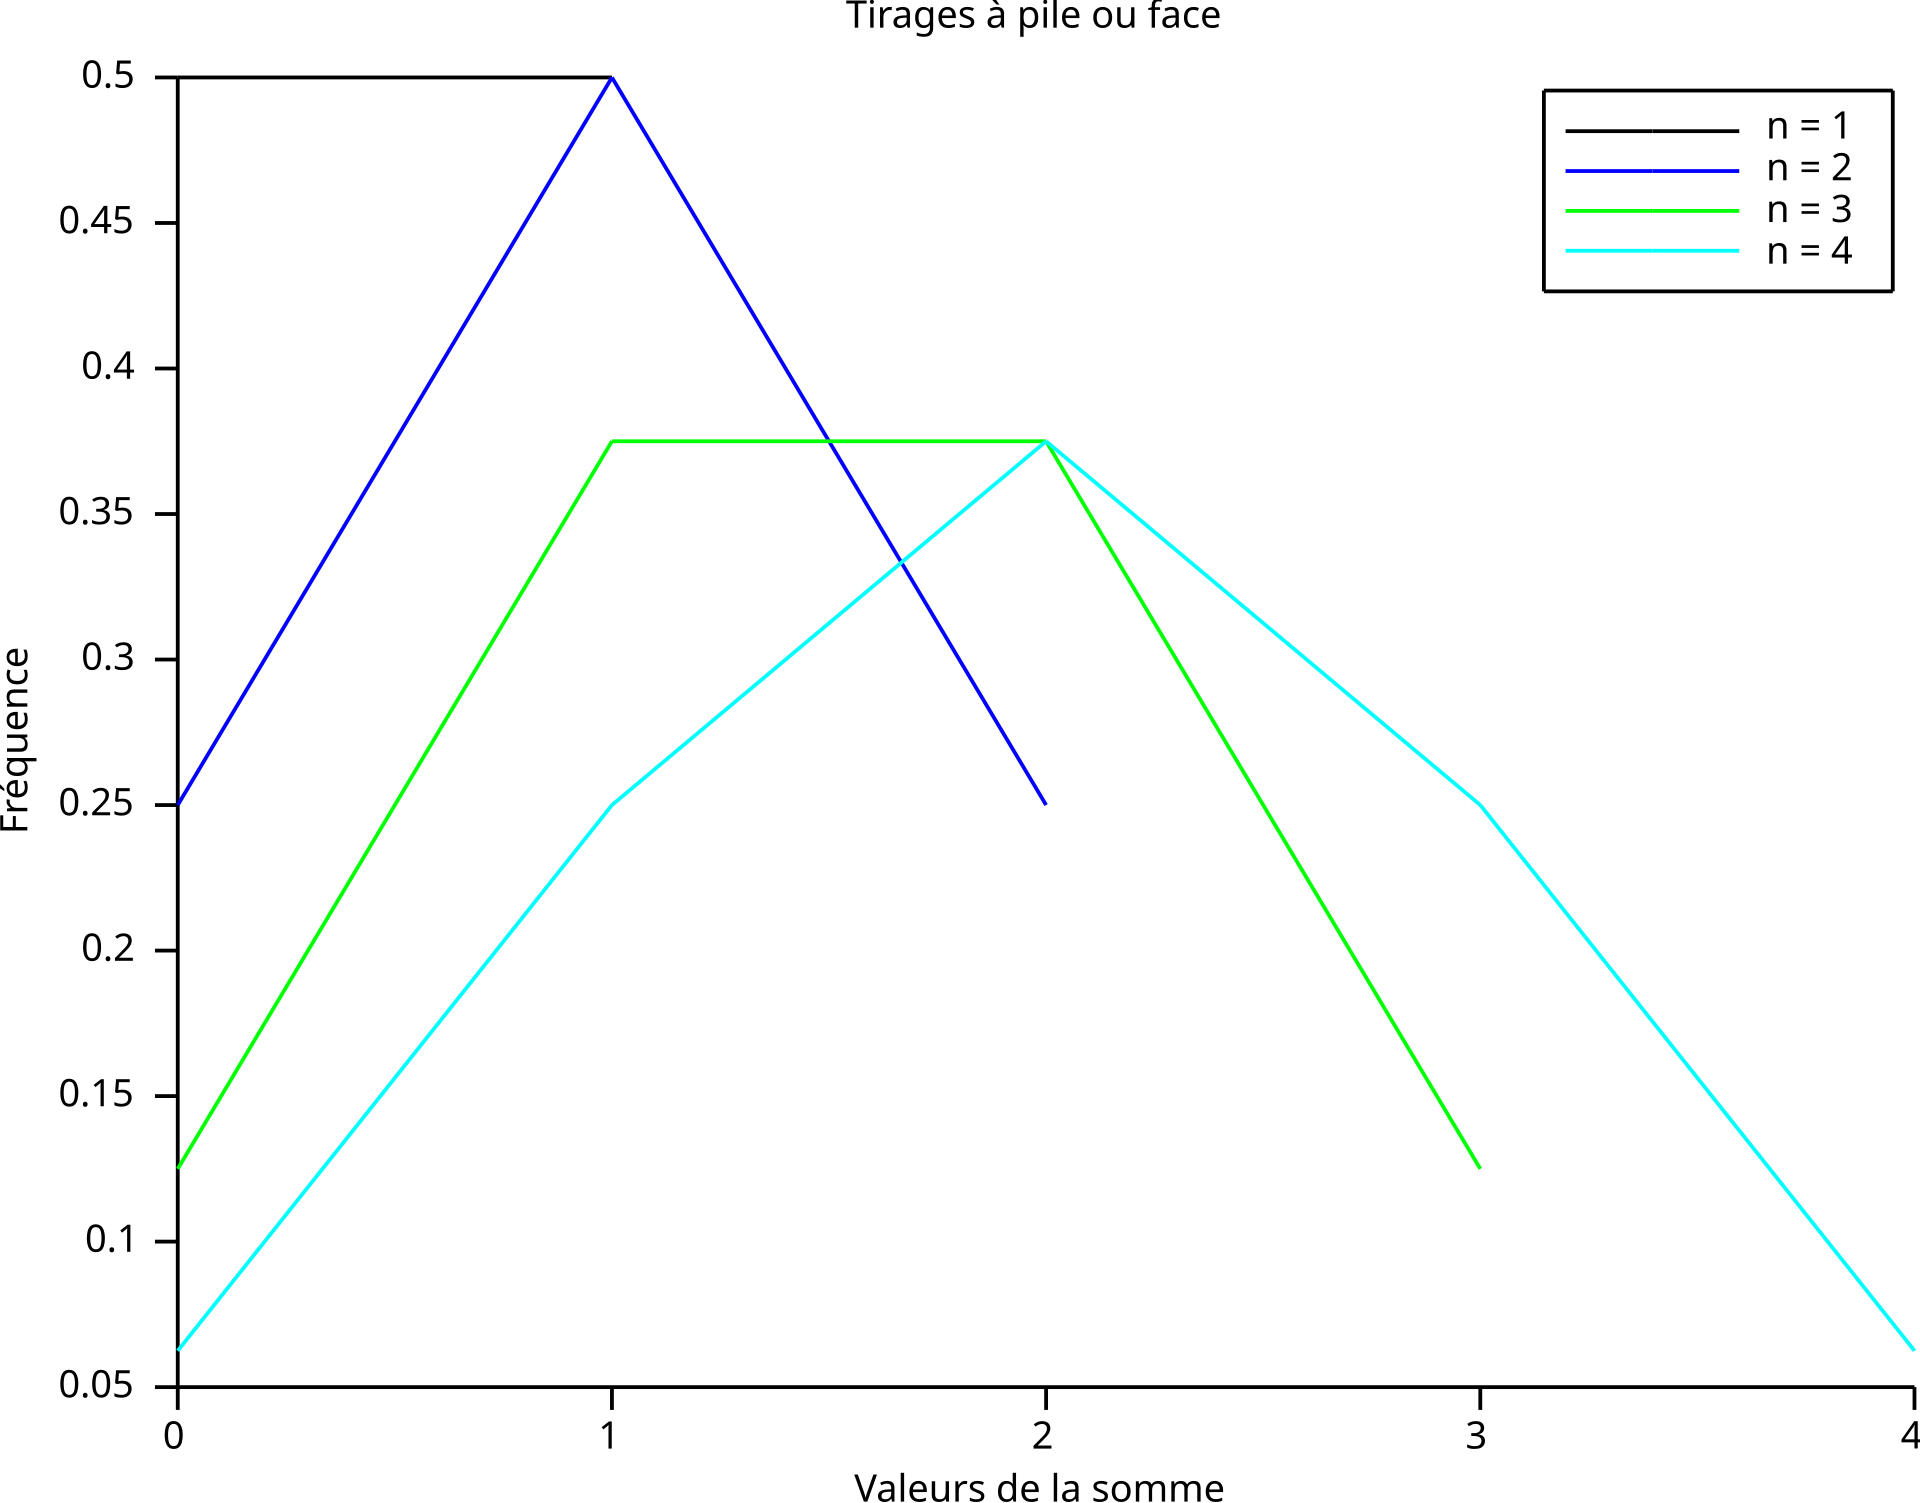
\includegraphics[width=0.7\textwidth]{images/courbe_tirages.png}
        \caption{Fréquence d'apparition d'une valeur pour la somme de $1 \leqslant n \leqslant 4$ tirages}
    \end{subfigure}
    \hfill
    \begin{subfigure}[b]{0.45\textwidth}
        \centering
        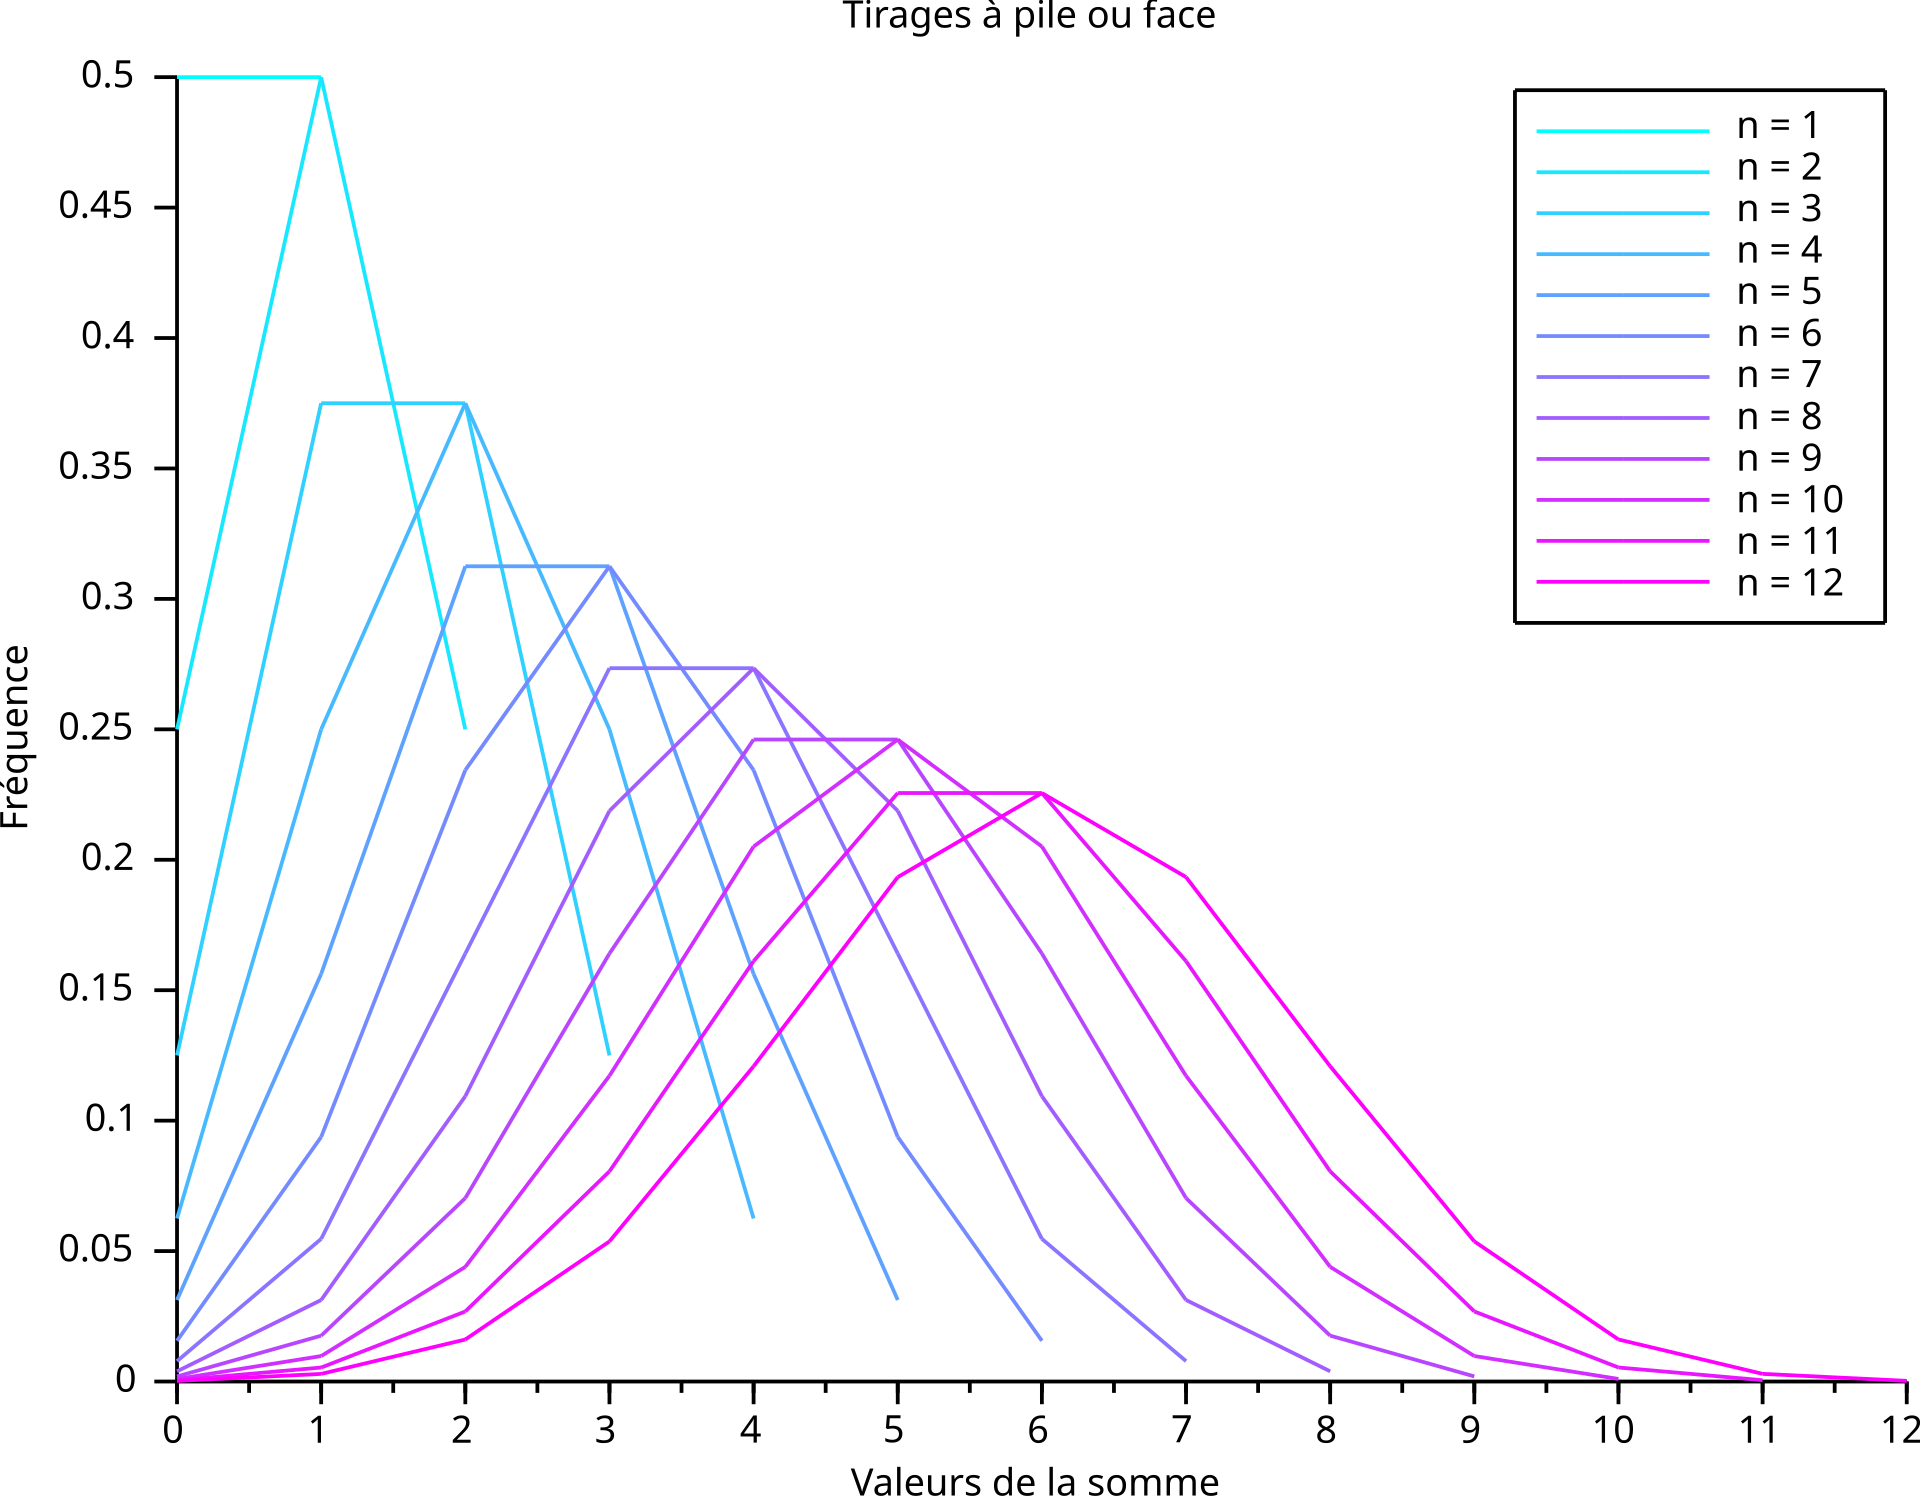
\includegraphics[width=0.7\textwidth]{images/courbe_tirages_12.png}
        \caption{\emph{Idem} pour $1 \leqslant n \leqslant 12$ tirages}
    \end{subfigure}
    \caption{Évolution de la fréquence d'apparition des sommes selon le nombre de tirages}
\end{figure}

Et cela pour n'importe quelle suite d'expériences aléatoires \emph{i.i.d}, la fréquence des sommes des issues obtenues 
"tend" vers la loi normale graphiquement. On peut interpréter de façon plus intuitive cette distribution. 
En effet, on peut se dire qu'il existe plus de façon d'effectuer un lancer qui se rapproche de la moyenne (centre de la courbe)
plutôt qu'un lancer improbable (aux extrémitées de la courbe). D'où cette distribution en cloche. 

\subsection{Théorème Central Limite}

Formalisons et généralisons ce que nous venons de voir avec un exemple. 

\begin{theorem}[Central Limite]
    Soit $(X_n)_{n \in \N^*}$ une suite de variables aléatoires \emph{i.i.d} admettant une moyenne et 
    une espérance telles que : 
        \[ \mu = \E(X_1) \quad \sigma^2 = \V(X_1) \] 
    Posons $S_n$ la somme des $n$ premières variables de la suite et $Y_n$ la variable centrée réduite de cette somme : 
        \[ S_n = X_1 + \dots X_n \quad \text{et} \quad Y_n = \frac{S_n - n \mu}{\sigma \sqrt{n}} \]
    Alors la suite $(Y_n)$ converge en loi vers la variables aléatoire de loi $ \mathcal{N}(0,1)$ 
    (la loi normale centrée réduite) :
        \[ \text{i.e } \quad \forall x \in \R, \quad \myP(Y_n \leqslant x) \underset{n \to \infty}{\longrightarrow} \frac{1}{\sqrt{2 \pi}} \int_{- \infty}^{x} e^{-u^2/2} \; du \] 
\end{theorem}






\end{document}